%{{{ preamble
\documentclass[a4paper,9pt]{article}
\usepackage{anysize}
\marginsize{2cm}{2cm}{1cm}{1cm}
%\textwidth 6.0in \textheight = 664pt
\usepackage{xltxtra}
\usepackage{xunicode}
\usepackage{graphicx}
\usepackage{color}
\usepackage{xgreek}
\usepackage{fancyvrb}
\usepackage{minted}
\usepackage{listings}
\usepackage{enumitem} 
\usepackage{framed} 
\usepackage{relsize}
\usepackage{float} 
\usepackage{pstricks}
\usepackage{pst-node}
\usepackage{pst-blur}
\setmainfont[Mapping=tex-text]{FreeSerif}
%}}}
\begin{document}

\def\thesection {\Roman{section}.}

\begin{titlepage}
\begin{center}
\begin{figure}[h] 
     
\includegraphics[width=0.2\textwidth]{title/ntua_logo}
\end{figure}
\vspace{1cm}
\begin{LARGE}\textbf{ΕΘΝΙΚΟ ΜΕΤΣΟΒΙΟ ΠΟΛΥΤΕΧΝΕΙΟ\\[1.5cm]}\end{LARGE}
\begin{Large}
ΣΧΟΛΗ ΗΜ\&ΜΥ\\
Δίκτυα Επικοινωνιών\\[2cm]
4\textsuperscript{η} Άσκηση\\
Ακ. έτος 2011-2012\\
\end{Large}
\vfill
\begin{flushright}
\begin{tabular}{l r}
{Γρηγόρης \textsc{Λύρας}}&
{Α.Μ.: 03109687}\\
\end{tabular}
\end{flushright}

\large\today\\
\end{center}
\end{titlepage}




\section*{Aνάλθση αποτελεσμάτων με τη βοήθεια του NAM}
Αρχικά χρησιμοποιήσαμε τον κώδικα που μας δίνεται από την εκφώνηση:

\inputminted[fontsize=\footnotesize]{tcl}{files/ex1_1.tcl}


Τρέχουμε το animation και παρατηρούμε την εξέλιξη της πορείας μετάδοσης των
πακέτων:

\begin{itemize}
    \item Με τη βοήθεια του animation παρατηρούμε πως η αποστολή των 50
    πακέτων από τον κόμβο 0 στον κόμβο 3 (Go back N protocol window 7) ολοκληρώνεται τη
    στιγμή 1.3sec. Από την άλλη πλευρά το τελευταίο πακέτο από τον κόμβο 1
    στον κόμβο 2 (Stop and Wait protocol window 1) φτάνει τη χρονική στιγμη
    5.6sec.
    \item $\frac{2Mb}{1040*8bits}\aprox240packets$
\end{itemize}

\begin{figure}[H]
    \centering
    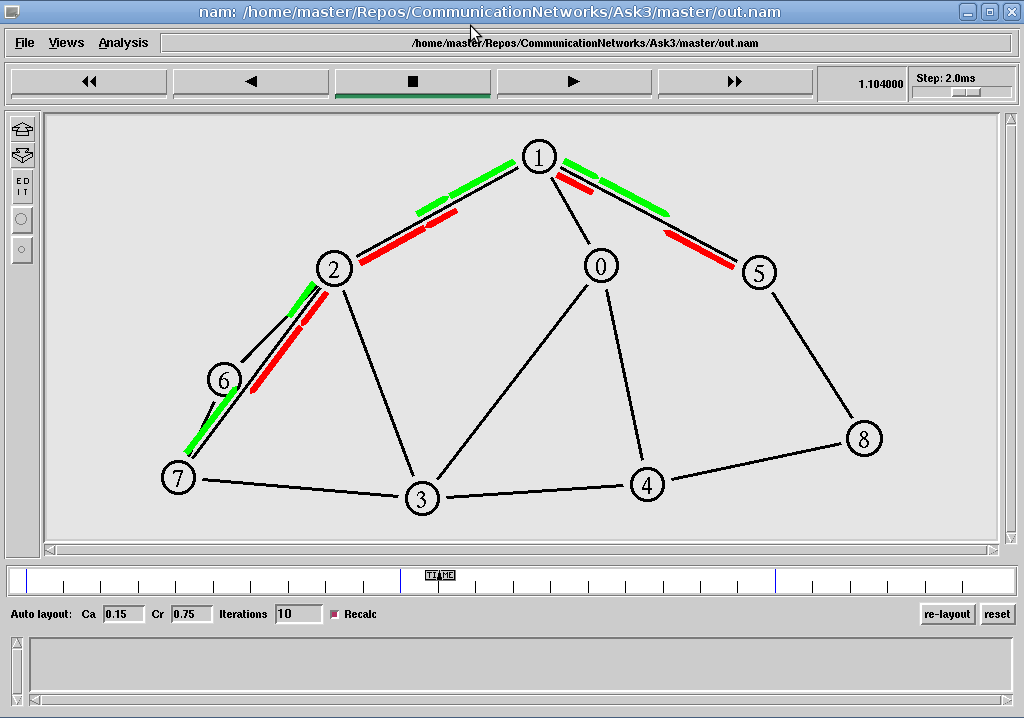
\includegraphics[width=0.8\textwidth]{files/2.png}
\end{figure}

Τα πακετα ακολουθουν τη διαδρομή (5 -> 1 ->  2 -> 7)
για να φτιάσουν στον προορισμό τους. Η διαδρομη αυτη ειναι η συντομοτερη
δυνατη. Ακολουθείται και κατά τις δύο κατευθύνσεις και δεν υπάρχει συντομότερη
διαδρομή με την παρούσα συνδεσμολογία μιας και το κόστος στις ζεύξεις είναι
ίσο και σταθερό.


\inputminted[fontsize=\footnotesize]{tcl}{files/ex3_1.tcl}
\section{}
Σε αυτήν ενότητα θα δούμε τη διαφορά μεταξύ στατικής και δυναμικής
δρομολόγησης και την εκάστοτε αντιμετώπιση από το δίκτυο. Μεταβάλλουμε λίγο
τον κώδικα, διακόπτοντας την σύνδεση ανάμεσα σε 1 και 2 για 0.4sec.

\inputminted[fontsize=\footnotesize]{tcl}{files/ex3_2.tcl}

\begin{figure}[H]
    \centering
    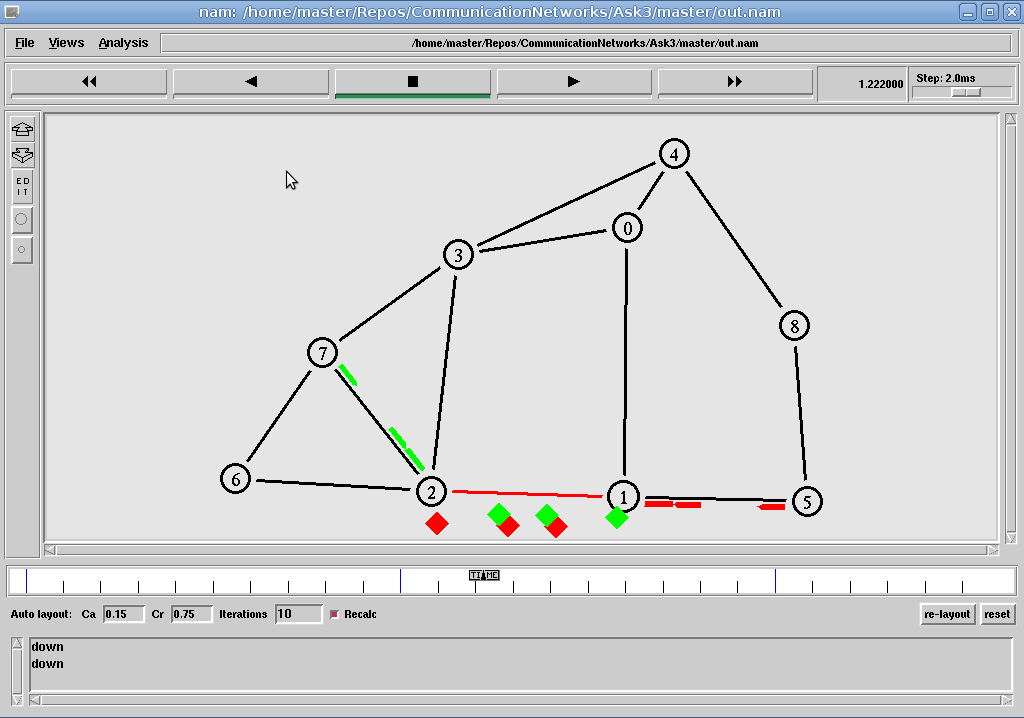
\includegraphics[width=0.8\textwidth]{files/3.png}
    \caption{Για χρόνο 1.2sec η σύνδεση διακόπτεται στη ζεύξη 1-2.}
\end{figure}


Προκειμένου να διορθώσουμε το παραπάνω πρόβλημα, αλλάζουμε τη σύνδεση σε
δυναμική με την ακόλουθη εντολή:
\begin{minted}[fontsize=\footnotesize]{tcl}
    $ns rtproto DV
\end{minted}

Παρατηρούμε ορισμένες αλλαγές σε σχέση με πριν. Αρχικά, εξετάζεται με
δοκιμαστικά πακέτα η συνδεσιμότητα των γραμμών:
\begin{figure}[H]
    \centering
    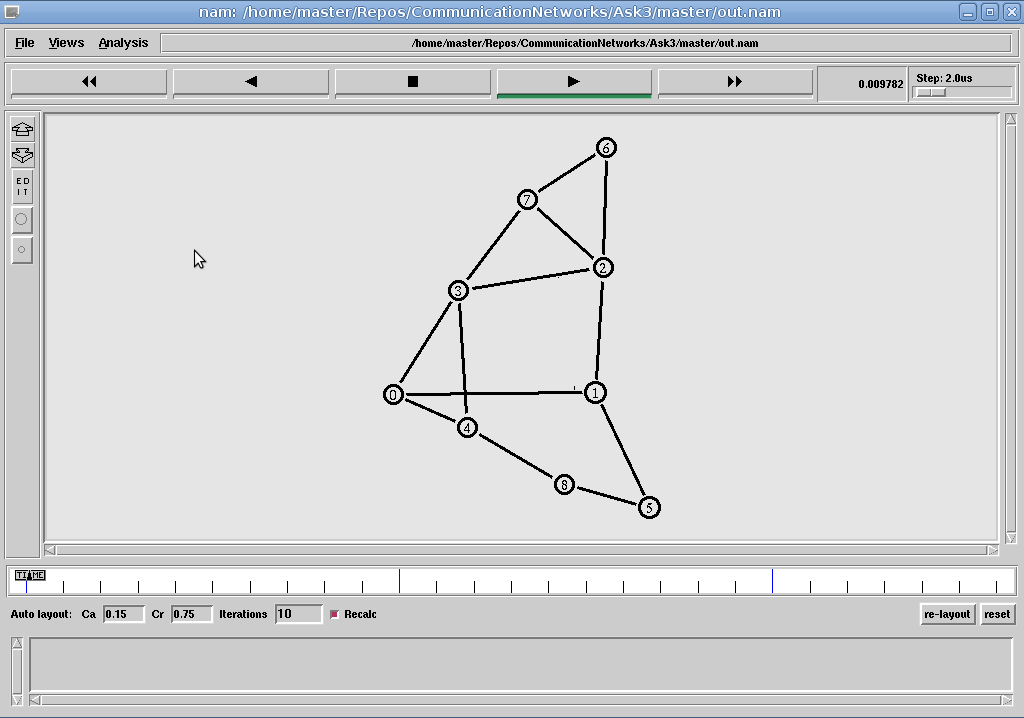
\includegraphics[width=0.8\textwidth]{files/4.png}
\end{figure}

Μετά τη διακοπή της σύνδεσης 1-2 επιλέγεται εναλλακτική διαδρομή, όταν
παρατηρείται η πρώτη απώλεια πακέτων:

\begin{figure}[H]
    \centering
    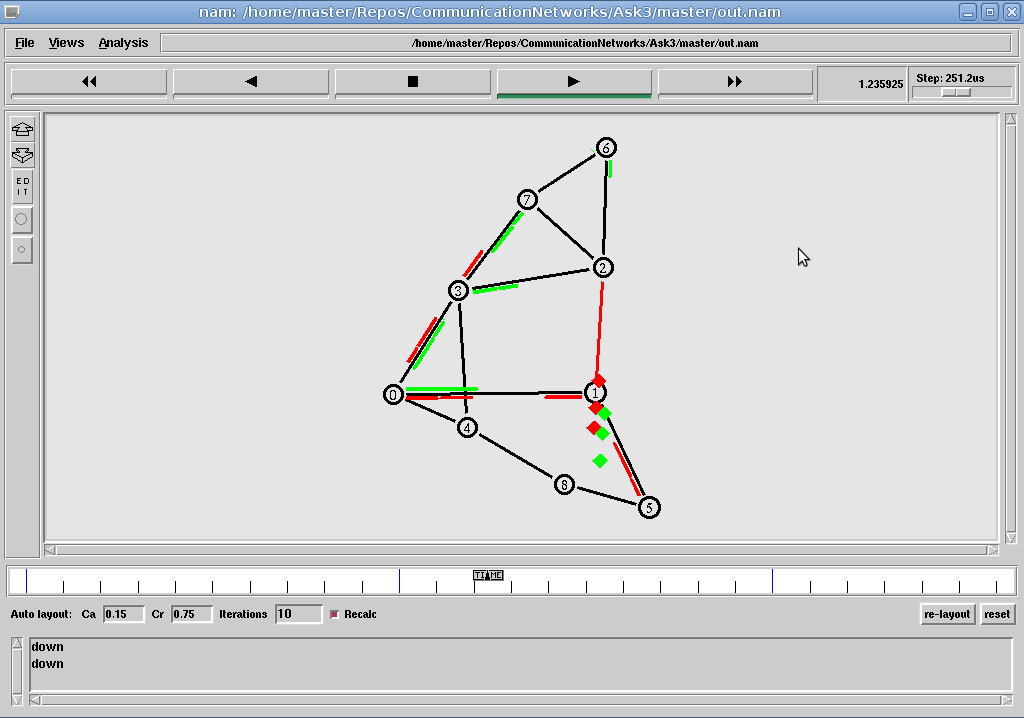
\includegraphics[width=0.8\textwidth]{files/5.png}
\end{figure}

Τέλος, μόλις η σύνδεση ενεργοποιηθεί ξανά, αρχίζει και πάλι η μετάδοση πακέτων
από αυτή. Ασφαλώς υπάρχει και ένας χρόνος που μεσολαβεί κατά τον οποίο και οι
δύο διαδρομές έχουν πακέτα.

\begin{figure}[H]
    \centering
    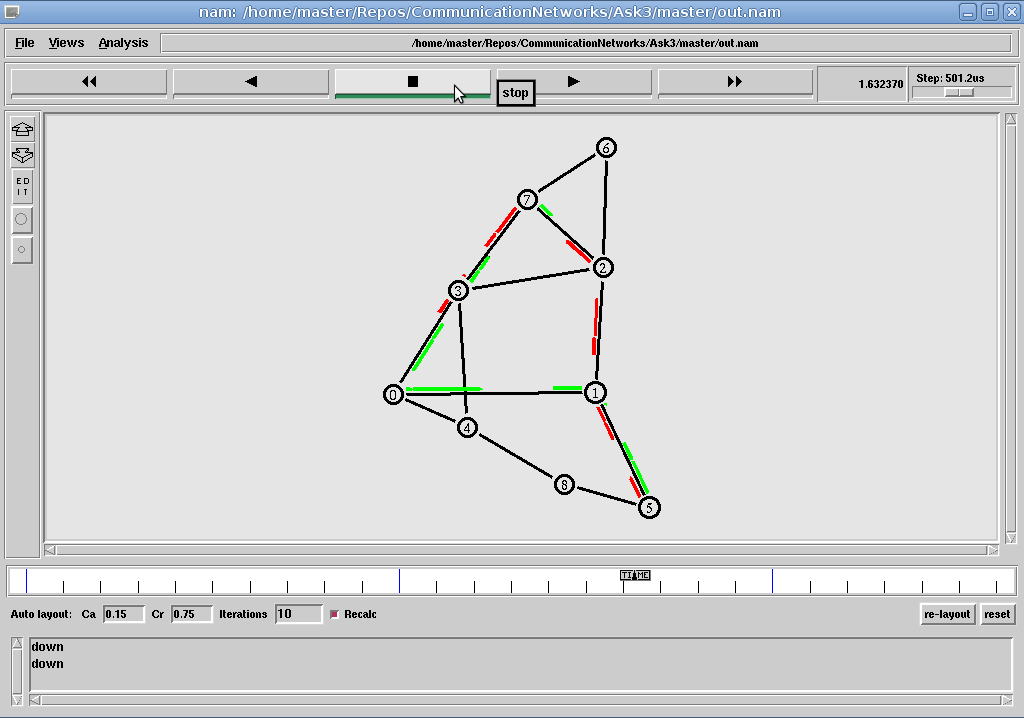
\includegraphics[width=0.8\textwidth]{files/6.png}
\end{figure}

\begin{itemize}
    \item Εξηγείστε γιατί με τη στατική δρομολόγηση, οι κόμβοι εξακολουθούν να
        στέλνουν πακέτα μετά τη διακοπή της ζεύξης.

        Καθώς, η δρομολόγηση είναι στατική, δεν ενημερώνονται οι κόμβοι με κανένα
        τρόπο για τη διακοπή της σύνδεσης. Επομένως δεν υπάρχει κάποια ανατροφοδότηση
        που θα τους οδηγούσε σε σχεδιασμό νέας διαδρομής.

    \item Τα πακέτα που χάνονται θα ξαναμεταδοθούν από τους αντίστοιχους κόμβους,
        όταν επανέλθει η σύνδεση;

        Αφού δεν υπάρχει ενημέρωση σχετικά με την απώλεια τους, ασφαλώς και οι κόμβοι
        δεν έχουν καμία πληροφορία για το αν χάθηκαν πακέτα και ποια είναι αυτά. Οπότε
        τα συγκεκριμένα πακέτα δε θα μεταδοθούν ξανά όταν επανέλθει η σύνδεση.

    \item Τι παρατηρείτε όταν γίνεται διακοπή ζεύξης και έχουμε δυναμική
        δρομολόγηση; 

        Περιγράψτε με απλά λόγια τη διαδικασία που λαμβάνει χώρα στο animation.
        Στη δυναμική δρομολόγηση, υπάρχει διαρκής ενημέρωση σχετικά με τη
        συνδεσιμότητα της κάθε γραμμής με τη βοήθεια βοηθητικών πακέτων. Αρχικά
        επιλέγεται η διαδρομή 5-1-2-7 που είναι και η συντομότερη. Μόλις κοπεί η
        σύνδεση 1-2, αμέσως βρίσκεται η συντομότερη διαδρομή που δε χρησιμοποιεί την
        αποσυνδεμένη ζεύξη. Αυτή είναι η 5-1-0-3-7. Προφανώς η διαδρομή αυτή είναι πιο
        αργή από την πρώτη. Για αυτό το λόγο, μόλις ενεργοποιηθεί ξανά η γραμμή 1-2,
        αυτόματα η μεταφορά πακέτων αρχίζει να ξαναγίνεται από εκεί.

    \item Ποιος από όλους τους κόμβους καθορίζει από ποια διαδρομή θα προωθηθούν
        κάθε φορά τα πακέτα;

        Αρχικά η πληροφορία για τη συνδεσιμότητα φθάνει στους κόμβους που έχουν επαφή
        με την αποσυνδεμένη ζεύξη και εκεί επανακαθορίζεται η διαδρομή που θα
        ακολουθηθεί για τον τελικό προορισμό. Σταδιακά η πληροφορία αυτή μεταβιβάζεται
        και στους γειτονικούς κόμβους και μόλις φτάσει στον αρχικό κόμβο, αυτός
        υπολογίζει ξανά τη διαδρομή λαμβάνοντας υπ’ όψιν τις αποσυνδεμένες ζεύξεις.
    \item Για ποιο λόγο τα πακέτα ακολουθούν τις συγκεκριμένες διαδρομές αφότου
        πέσει η σύνδεση;

        Ο λόγος που γίνεται αυτό είναι επειδή οι συγκεκριμένες διαδρομές είναι οι
        συντομότερες για τον προορισμό που δεν χρησιμοποιούν την κομμένη ζεύξη. Επί
        της ουσίας, επανασχεδιάζεται η διαδρομή στον κόμβο που εντοπίζεται η διακοπή
        ζεύξης και, όταν η πληροφορία φτάσει στον αρχικό κόμβο σε αυτόν, για να βρεθεί
        ο συντομότερος τρόπος ώστε να προσεγγιστεί ο προορισμός χωρίς αυτή τη σύνδεση.
    \item Θα μπορούσαν να δρομολογηθούν από άλλους κόμβους;

        Ασφαλώς η δρομολόγηση θα μπορούσε να γίνει και από άλλους κόμβους, με
        μεγαλύτερο πλήθος κόμβων να διαρρέεται αλλά κάτι τέτοιο είναι χρονοβόρο χωρίς
        να προσφέρει επί της ουσίας κάτι.
\end{itemize}


\section{}
Σε αυτό το κομμάτι της άσκησης αλλάζουμε το κόστος των διαδρομών όπως φαίνεται
στον κώδικα παρακάτω.

\inputminted[fontsize=\footnotesize]{tcl}{files/ex3_3.tcl}

Εκτελώντας την προσομοίωση και πάλι παρατηρούμε ότι πλέον όταν κόβεται η ζεύξη
1-2 επιλέγεται διαφορετική πορεία από πριν. Καθώς  αυτή τη φορά
συνοπολογίζουμε και το διαφορετικό κόστος κάθε ζεύξης 5-0-3-7.

\begin{figure}[H]
    \centering
    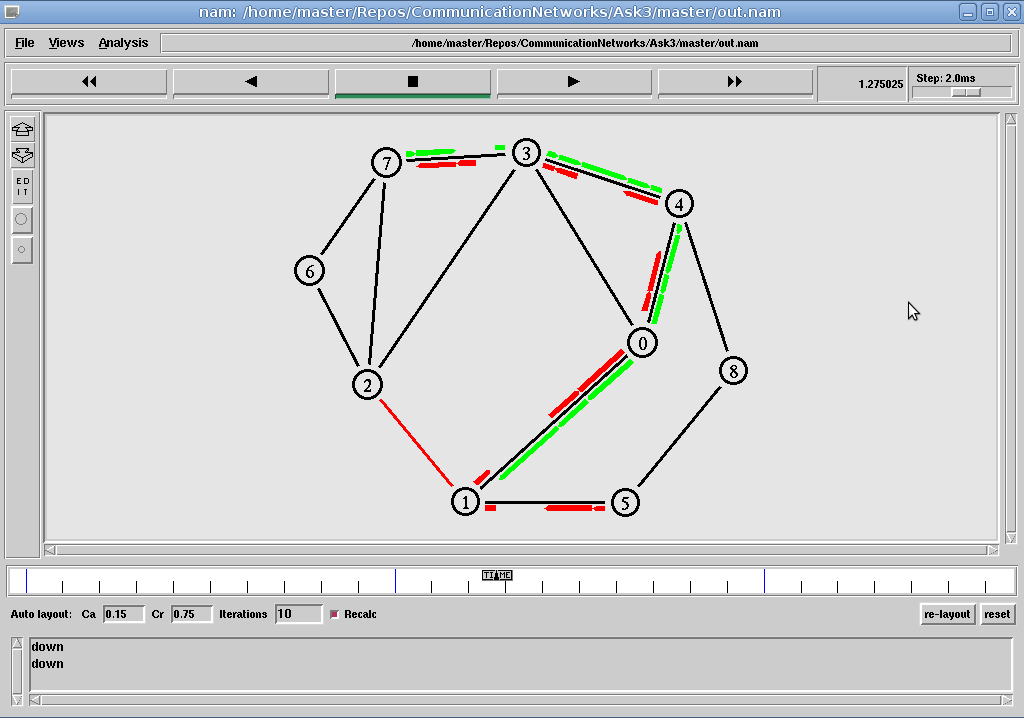
\includegraphics[width=0.8\textwidth]{files/8.png}
\end{figure}

\begin{itemize}
    \item Ποιές διαδρομές ακολουθούν τα πακέτα πριν , μετά και κατά τη διάρκεια της
        πτώσης της σύνδεσης;

        Τα πακέτα όπως ήταν αναμενόμενο ακολουθούν πριν και μετά την πτώση της
        σύνδεσης 1-2 την ίδια διαδρομή με τα προηγούμενα ερωτήματα. Κατά τη διάρκεια
        της πτώσης επιλέγουν η διαδρομή 5-1-0-4-3-7 .

    \item Για ποιόν λόγο τα πακέτα ακολουθούν τις συγκεκριμένες διαδρομές;

        Ο λόγος για τον οποίο τα πακέτα ακολουθούν τις παραπάνω διαδρομές είναι ότι με
        βάση τα βάρη που έχουν οι ζεύξεις, αυτές είναι οι διαδρομές που κοστίζουν
        λιγότερο.

    \item Θα μπορούσαν να δρομολογηθούν από άλλους κόμβους;

        Προφανώς θα μπορούσαν να δρομολογηθούν από άλλους κόμβους τα πακέτα (βλ. Μέσω
        του κόμβου 8) αλλά αυτό θα ήταν ακριβότερο γι’αυτό επιλέγεται η παραπάνω
        διαδρομή.
\end{itemize}



\section{}


Προσθέτουμε τις κατάλληλες εντολές και ο τελικός κώδικας διαμορφώνεται όπως
φαίνεται παρακάτω. Σβήνουμε τις εντολές που προκαλούν τη διακοπή της σύνδεσης
όταν t=1.2sec  και την αποκατάστασή της όταν t=1.6sec ώστε να μην υπάρχουν
προβλήματα στη ροή δεδομένων. Ακόμη ρυθμίζουμε το χρόνο προσομοίωσης στα 15sec
ώστε να έχουμε αντιπροσωπευτικά αποτελέσματα.

\subsection{CBR}
\inputminted[fontsize=\footnotesize]{tcl}{files/ex3_4a1.tcl}

\begin{figure}[H]
    \centering
    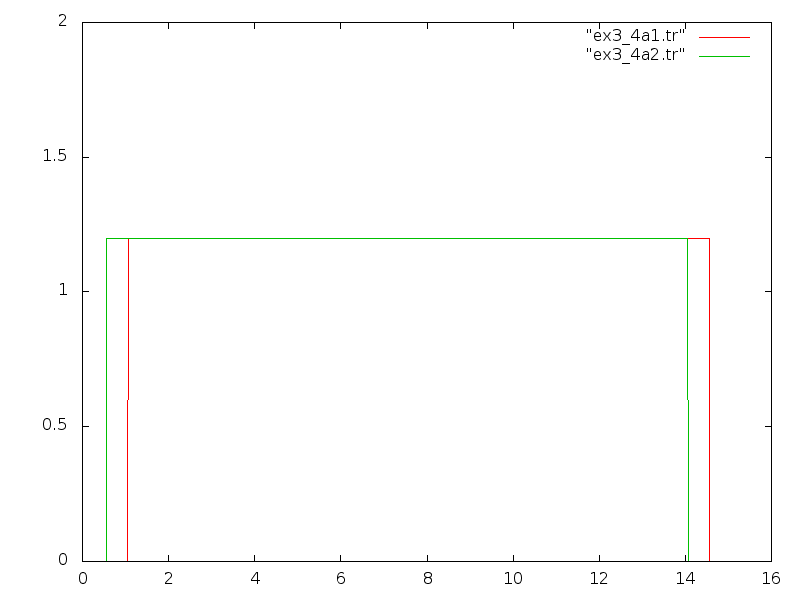
\includegraphics[width=0.7\textwidth]{files/graph1.png}
\end{figure}

\subsection{Exponential}
\inputminted[fontsize=\footnotesize]{tcl}{files/ex3_4a2.tcl}
\begin{figure}[H]
    \centering
    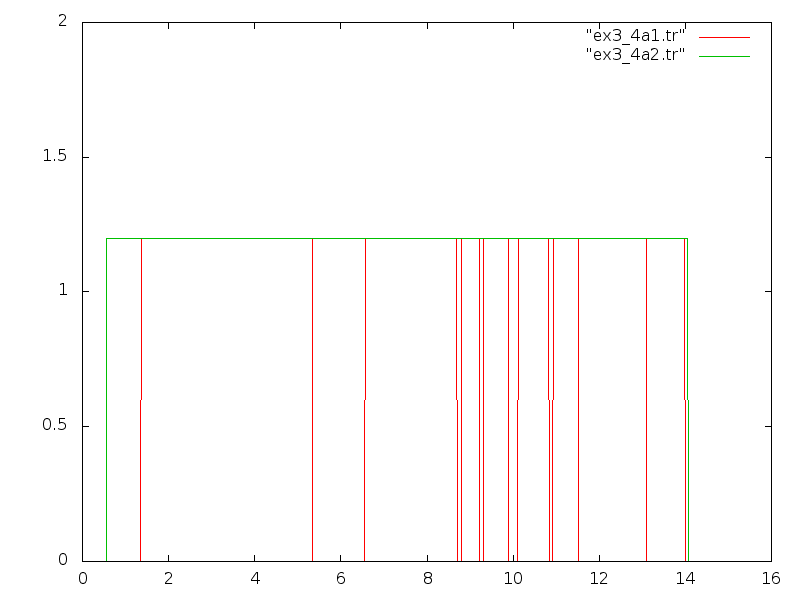
\includegraphics[width=0.7\textwidth]{files/graph2.png}
\end{figure}

\begin{itemize}
    \item Ποιός είναι ο μέγιστος αριθμός μετάδοσης που επιτυχγάνεται για τις δύο
        περιπτώσεις κίνησης, με βάση τις γραφικές παραστάσεις που σχεδιάσατε;

        Ο μέγιστος ρυθμός μετάδοσης είναι και για τις δύο περιπτώσεις κίνησης 0.18.
    \item Αιτολογήστε τις τιμές που θέσατε παραπάνω για τις δύο τιμές κίνησης (cbr
        και exp);

        H παραπάνω τιμή είναι λογική αφού είναι ελαφρώς μικρότερη από το εύρος ζώνης
        της σύνδεσης (δηλ 2Mb).
\end{itemize}


\end{document}

